\documentclass{standalone}
\usepackage{chez}

\begin{document}
\chapter{October 05, 2020}

\begin{proposition}
  Suppose \(X\) is a CW complex and \(k, q, \geq 0\), then
    \(H_q(\Sk_k X) \iso 0\) for \(k < q\) and
    \(H_q(\Sk_k X) \iso H_q(X)\) for \(k > q\).
\end{proposition}
\begin{example}
  If \(q = 0\), then \(H_0(\Sk_k X) \iso H_0(X)\) for \(k > 0\).
  For example, if we had the following skeleta,
  \begin{center}
    \setlength{\tabcolsep}{4em}
    \begin{tabular}{c c c}
      \(\Sk_0 X\) & \(\Sk_1 X\) & \(\Sk_2 X\) \\
      \begin{tikzpicture}
        \fill (0, 0) circle[radius=0.05];
        \fill (2, -1/2) circle[radius=0.05];
        \fill (2, 1/2) circle[radius=0.05];
      \end{tikzpicture}
      &
      \begin{tikzpicture}
        \fill (0, 0) circle (0.05);
        \fill (2, -1/2) circle (0.05);
        \fill (2, 1/2) circle (0.05);
        \draw (2, -1/2) to[bend left] (2, 1/2);
        \draw (2, -1/2) to[bend right] (2, 1/2);
      \end{tikzpicture}
      &
      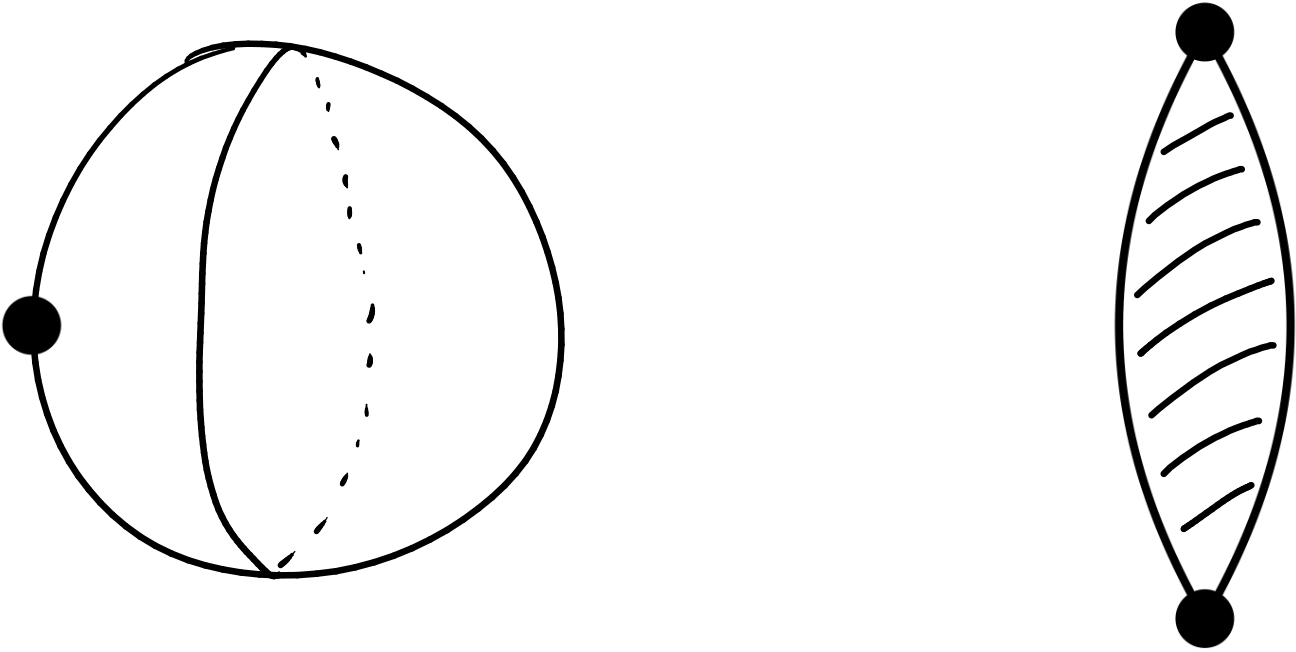
\includegraphics[height=1.2cm]{18_905-201005-1.png}
    \end{tabular}
  \end{center}
  note that attaching a \(k\)-cell (\(k > 1\)) to objects already present
  cannot change the number of path components, which is exactly what the
  proposition says.

  If \(q = 1\), then we have
  \begin{itemize}[nosep]
    \item \(H_1(\Sk_0 X) \iso 0\),
    \item \(H_1(\Sk_1 X)\) is something,
    \item \(H_1(X) \iso H_1(\Sk_2 X) \iso H_1(\Sk_3 X) \iso \cdots\)
  \end{itemize}
  In particular, we have \(H_1(\Sk_1 X) \iso \ZZ\),
  and \(H_1(\Sk_2 X) \iso 0\).
\end{example}

Intuitively, when we add the \(k\)-dimensional cells, we are adding cycles.
But when we compute homologies, we mod out by the boundaries,
which are added when \((k+1)\)-cells are added.
In particular, once \((k+1)\)-cells are added,
higher dimensional cells will not affect \(H_k\).

In general, we have
\begin{itemize}
  \item \(H_q(\Sk_{q-1} X) \iso 0\),
  \item \(H_q(\Sk_q X)\) surjects onto \(H_q(X)\), and
  \item \(H_q(\Sk_{q+1} X) \iso H_q(X)\).
\end{itemize}

\begin{proof}
  To compare \(H_q(\Sk_{k-1} X)\) and \(H_q(\Sk_k X)\),
  we can use the long exact sequence of the pair \((\Sk_k X, \Sk_{k-1} X)\).
  
  The key idea is that
  \[
    H_q(\Sk_k X, \Sk_{k-1} X)
      \iso \tilde H_q \parens{\Sk_k X / \Sk_{k-1} X}
      \iso \tilde H_q \parens[\Big]{\bigvee_{i \in I_k} S^k}
      \iso \begin{cases*}
        \bigoplus_{i \in I_k} \ZZ & if \(q = k\) \\[-1ex]
        0 & otherwise.
      \end{cases*}
  \]
  The long exact sequence of pairs gives
  \(H_q(\Sk_k X) \iso 0\) if \(k < q\)
  because for sufficiently small \(k\), \(H_q(\Sk_k X) \iso H_q(\Sk_{k-1} X)\).
  The long exact sequence also gives
  \(H_q(\Sk_k X) \iso H_q(\Sk_{k+1} X)\) if \(k > q\).
  It remains to check that
  \[
    H_q(\Sk_k X) \simeq H_q(X)
  \]
  if \(k = q\).
  Note that \(\Delta^q\) and \(\Delta^{q+1}\) are compact,
  so anything in \(H_q(X)\) has to be represented by
  a finite linear combination of simplices,
  which by compactness has to be contained in some finite skeleton.
  Knowing \(\Delta^q\) is compact tells us that
  \(H_q(X) \to H_{q+1(X)}\) is surjective,
  and knowing that \(\Delta^{q+1}\) is compact tells us that
  the boundary relations are present as well.
\end{proof}


\section{Cellular homology}
Now we will introduce a tool to compute homology groups.
\begin{definition}
  Suppose \(X\) is a CW complex.
  Let \(C_n(X) = C_n^{\text{cell}}(X)\) denote
  \[
    H_n(\Sk_n X, \Sk_{n-1} X) \simeq
      \tilde H_n \parens[\Big]{\bigvee_{i \in I_n} S^n},
  \]
  the free abelian group on the set of \(n\)-cells of \(X\).
\end{definition}

\begin{definition}
  For each \(n \geq 0\), we can define the map
  \[
    d \colon C_{n+1}(X) \to C_n(X)
  \]
  to be the composite
  \[
    \begin{tikzcd}
      C_{n+1}(X) = H_{n+1}(\Sk_{n+1} X, \Sk_n X) \ar[r, "\partial"] &
      H_n(\Sk_n X) \ar[r] &
      H_n(\Sk_n X, \Sk_{n-1} X) = C_n(X)
    \end{tikzcd}
  \]
\end{definition}

\begin{theorem}
  The maps \(d \colon C_{n+1}(X) \to C_n(X)\) make \(C_*(X)\) into
  a chain complex (i.e.\ \(d \circ d = 0\)).
  The homology of this chain complex is isomorphic to the homology of \(X\).
  This is called \vocab{cellular homology}.
\end{theorem}

Consider the sequence of functors
\[
  \begin{tikzcd}
    \Fun(\Deltainj^\op, \cSet) \ar[r, "F"] &
    \cCWcomp \ar[r, "U"] &
    \cTop
  \end{tikzcd}
\]
i.e.\ the geometric realization of a semisimplicial set.
Then \(C_n^{\text{cell}}(F(X)) = \ZZ \Sing_n X = S_n(X)\)
and \(C_*^{\text{cell}}(F(X)) = S_*(X)\).
Thus, the theorem says that the semisimplicial homology of \(X\) agrees
with the singular homology of the geometric realization of \(X\).

\begin{example}[Homology of \(S^n\)]
  Recall that \(S^n\) has a very simple CW complex structure that requires
  one \(0\)-cell and one \(n\)-cell.
  Since \(C_l^{\text{cell}}(X)\) is the free abelian group on
  the set of \(l\)-cells, we have
  \[
    C_l^{\text{cell}}(S^n) = \begin{cases*}
      \ZZ & if \(l = 0, n\) \\[-1ex]
      0 & otherwise.
    \end{cases*}
  \]

  For e.g.\ \(n = 2\), we have the chain complex \(C_*(S^2)\) is isomorphic to
  \[
    \begin{tikzcd}
      \ZZ &
      0 \ar[l, "d"'] &
      \ZZ \ar[l, "d"'] &
      0 \ar[l, "d"'] &
      0 \ar[l, "d"'] &
      \cdots \ar[l, "d"']
    \end{tikzcd}
  \]
  Since most of these groups are \(0\), we can easily compute:
  \[
    H_0(S^2) \iso \ZZ \qquad
    H_1(S^2) \iso 0 \qquad
    H_2(S^2) \iso \ZZ \qquad
    H_3(S^2) \iso 0,
  \]
  i.e.\ \(H_q(S^2) \iso \begin{cases*}
    \ZZ & if \(q = 0, 2\) \\[-1ex]
    0 & otherwise.
  \end{cases*}\)
\end{example}

\begin{remark}
  If a CW complex only has even dimensional cells, then
  \[
    H_q(X) \iso \begin{cases*}
      \bigoplus_{i \in I_q} \ZZ & \(q\) is even \\[-1ex]
      0 & \(q\) is odd.
    \end{cases*}
  \]
\end{remark}

\begin{example}[Torus]<torus-cell-homology>
  The torus \(T^2\) has a CW structure
  \begin{align*}
    \Sk_0 T^2 &= * \\[-1ex]
    \Sk_1 T^2 &= \enskip 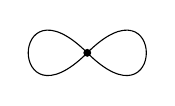
\begin{tikzpicture}[baseline, yshift=0.6ex]
      \fill (0, 0) circle (0.05);
      \draw (0, 0) .. controls (1/4, -1/4) and (7/16, -5/16) .. (9/16, -9/32);
      \draw (9/16, -9/32) .. controls (11/16, -1/4) and (3/4, -1/8) .. (3/4, 0);
      \draw (3/4, 0) .. controls (3/4, 1/8) and (11/16, 1/4) .. (9/16, 9/32);
      \draw (9/16, 9/32) .. controls (7/16, 5/16) and (1/4, 1/4) .. (0, 0);
      \begin{scope}[xscale=-1]
        \draw (0, 0) .. controls (1/4, -1/4) and (7/16, -5/16) .. (9/16, -9/32);
        \draw (9/16, -9/32) .. controls (11/16, -1/4) and (3/4, -1/8) .. (3/4, 0);
        \draw (3/4, 0) .. controls (3/4, 1/8) and (11/16, 1/4) .. (9/16, 9/32);
        \draw (9/16, 9/32) .. controls (7/16, 5/16) and (1/4, 1/4) .. (0, 0);
      \end{scope}
    \end{tikzpicture}
    \enskip = \begin{tikzpicture}[baseline, yshift=-3.4ex]
      \begin{scope}[decoration={markings, mark=at position 0.5 with {\arrow{>>}}}]
        \draw[postaction={decorate}] (0, 0) -- (1, 0) node[midway, below]{\(b\)};
        \draw[postaction={decorate}] (0, 1) -- (1, 1) node[midway, above]{\(b\)};
      \end{scope}
      \begin{scope}[decoration={markings, mark=at position 0.5 with {\arrow{>}}}]
        \draw[postaction={decorate}] (1, 0) -- (1, 1) node[midway, right]{\(a\)};
        \draw[postaction={decorate}] (0, 0) -- (0, 1) node[midway, left ]{\(a\)};
      \end{scope}
      \fill (0, 0) circle[radius=0.02];
      \fill (0, 1) circle[radius=0.02];
      \fill (1, 0) circle[radius=0.02];
      \fill (1, 1) circle[radius=0.02];
    \end{tikzpicture} \\ % chktex 31
    \Sk_2 T^2 &= \enskip\parbox{0.15\textwidth}{%
      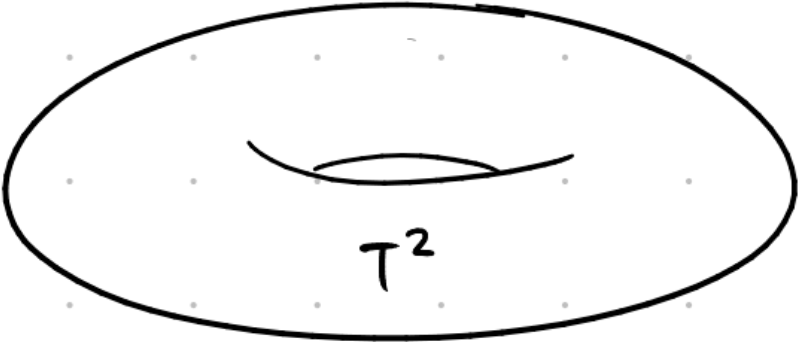
\includegraphics[width=0.15\textwidth]{18_905-201005-2-torus.png}}
  \end{align*}
  where the \(2\)-skeleton is obtained by attaching one \(2\)-cell
  via the map \(S^1 \to \Sk_1 T^2\) which is \(b\inv a\inv b a\).

  We can compute the homology group from the cellular chain complex
  \[
    \begin{tikzcd}
      \ZZ\fgen{x} &
      \ZZ\fgen{a, b} \iso \ZZ \oplus \ZZ \ar[l, "d_1"'] &
      \ZZ\fgen{u} \ar[l, "d_2"'] &
      0 \ar[l] &
      \cdots \ar[l]
    \end{tikzcd}
  \]
  Note that \(d_1\) has to be zero because the boundaries
  of \(a\) and \(b\) are the same point.
  To compute \(d_2\), note that the boundary of the \(2\)-cell \(u\)
  is glued on via \(b\inv a\inv b a\).
  Therefore,
  \[
    d_2 u = -b -a + b + a = 0.
  \]
  This gives the expected homology groups.
\end{example}

\begin{proof}[\(C_*^{\text{cell}}(X)\) agrees with singular homology]
  Consider the diagram
  \[
    \begin{tikzcd}
      & \mathllap{C_{n+1}^{\text{cell}}(X) = {}}
        H_{n+1}(\Sk_{n+1} X, \Sk_n X) \ar[d, blue, "\partial_n"] \ar[dr, "d"]
        & & H_{n-1}(\Sk_{n-2} X) \mathrlap{{} = 0} \ar[d] \\
      \mathllap{0 = {}} H_{n+1}(\Sk_{n-1} X) \ar[r]
        & H_n(\Sk_n X) \ar[r, blue, "j_n"] \ar[d]
        & H_n(\Sk_n X, \Sk_{n-1} X) \ar[r, blue, "\partial_{n-1}"] \ar[dr, "d"]
        & H_{n-1}(\Sk_{n-1} X) \ar[d, blue, "j_{n-1}"] \\
      & H_n(\Sk_{n+1} X) \ar[d]
        & & H_{n-1}(\Sk_{n-1} X, \Sk_{n-2} X) \\
      & \mathllap{0 = {}} H_n(\Sk_{n+1} X, \Sk_n X)
    \end{tikzcd}
  \]
  All of the rows and columns are exact.
  The theorem claims that \(d \circ d = 0\),
  and \(\ker d / \img d\) agrees with singular homology.

  To show that \(d \circ d = 0\), note that \(d \circ d\) is the same as
  following the blue arrows. However, the horizontal sequence is exact, so
  the composite of the two blue horizontal maps is zero.

  To show that \(\ker d / \img d\) computes singular homology,
  note that \(j_{n-1}\) is injective from exactness. Therefore,
  \(\ker d = \ker \partial_{n-1}\),
  and furthermore
  \(\ker d = \ker \partial_{n-1} = \img j_n\)
  by exactness of the horizontal sequence.
  We also have \(j_n\) is injective from exactness,
  so \(\img j_n \iso H_n(\Sk_n X)\).

  Therefore,
  \[
    \frac{\ker d}{\img d}
      = \frac{H_n(\Sk_n X)}{\img \partial_n}
      = H_n(\Sk_{n+1} X)
      = H_n(X). \pog
  \]
\end{proof}




\end{document}
